\pagebreak
\subsection{Software Design}
\subsubsection{Purpose}
The purpose of the software was to automate control of the valves so that they will be opened/closed at the target altitude. Moreover, the software stored housekeeping data from sensors, pump, and valves states to the on-board memory storage device. Logging sensor data was necessary in order to determine a vertical profile of the analyzed samples:

\begin{quote}
In order to determine the vertical profiles of CO$_2$, CH$_4$, and CO from the analysis of sampled air, measurements of several atmospheric parameters were needed [...]. The two most important parameters were the ambient pressure and the mean coil temperature. These parameters were be recorded by the AirCore-HR (High Resolution) electronic data package. Mean coil temperature was obtained by taking the mean of three temperatures recorded by independent probes located at different positions along the AirCore-HR.\cite{Membrive}
\end{quote}

Both the ambient pressure and the sampling container temperature were also essential for AAC sampling bags. The temperature data was collected by the sensors near the sampling bags.

The software shall also transmit data to the ground so that the team can monitor the conditions of the experiment in real time. Telecommand was also needed to overwrite pre-programmed sampling scheduled in case of automation failure or to mitigate unexpected changes in the flight path and reached altitudes. It was used to test the system, especially valves and heaters.\par

\subsubsection{Design} \label{sec:4.8.2}
\begin{enumerate}[label=(\alph*)]
\item{Process Overview}\\
The software which ran on the Arduino read from the sensors through the analog, I2C, and SPI interfaces. The sensors provided temperature, pressure and airflow data. The acquired data was time-stamped and stored in the on-board SD card and transmitted via the E-Link System to the ground station. Then according to the pressure/altitude, the software controlled the valves which allowed the air to be pumped inside the bags. Figure \ref{processOverview} visually explain the process flow.

\begin{figure}[H]
    \centering
    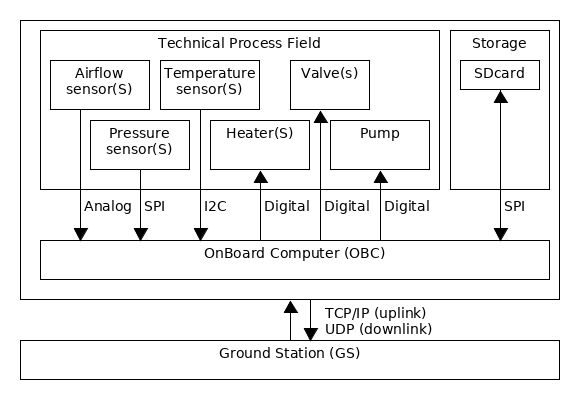
\includegraphics[width=0.85\textwidth]{4-experiment-design/img/Process-overview-V0-3.png}
    \caption{The Process Overview of the Experiment.}
    \label{processOverview}
\end{figure}

\item{General and Safety related concepts}\\
The watchdog timer, which was an electronic countdown timer that causes an interrupt when it reaches 0, was used to avoid failure because of a possible freezing problem in the software. During normal operations, the software set flags when done with their task. When all the flags had been set the watchdog got reset. If any task fails to set the their flag before the watchdog elapses, the system resets. Telecommand was also be used as backup in case the automation fails or otherwise become unresponsive. Telemetry was utilized to transmit housekeeping data and the state of the valves to get confirmation of operation. Rigorous testing was performed during the development of the project and before the launch phase to insure that that the software was capable to control the experiment.
\item{Interfaces}\\
Table \ref{tab:comIntpro} demonstrates how the components interacted with the onboard computer (OBC). Components that used SPI, shared MISO, MOSI, and CLK pins on the Arduino board. Each of them was also connected to general pins input output (GPIO) for slave select. Furthermore, components using I2C protocol, shared Serial Data pin (SDA) and Serial Clock pin (SCL).

\begin{table}[H]
\centering
\begin{tabular}{lll}
Components interacting & Communication protocol & Interface                 \\ \hline
Pressure Sensors-OBC   & SPI                    & Arduino SPI and Digital Pins \\
Temperature sensors-OBC        & I2C                    & Arduino I2C \\
Airflow sensor-OBC     & I2C                    & Arduino I2C \\
Heaters-OBC            & Digital                & GPIO pins \\
Air pump-OBC           & Digital                & GPIO pins \\
Valve-OBC              & Digital                & GPIO pins                 \\
OBC-microSD Storage    & SPI                    & Arduino Ethernet shield   \\
OBC - E-Link           & Ethernet               & Ethernet port            
\end{tabular}%Tabular dude
\caption{Communication and interface protocols}
\label{tab:comIntpro}
\end{table}

Every transmission to/from the ground utilized the E-link connection. The data packet which was used was an Ethernet Packet with a header containing the address of destination, followed by the data, and at the end there was a frame check sequence (FCS). The up-linked data packet had the same structure, with header followed by commands and ended with FCS.\\
\\
The protocol that had been chosen was UDP for telemetry and TCP for telecommand. The UDP was used to prevent software getting stuck waiting for handshake from the ground if the connection was temporarily lost.\\
\\
The telecommand contained the following services:
\begin{itemize}
    \item Changing instrument modes
    \item Manually control valves, pump, and heaters
    \item Change sampling schedule
\end{itemize}

Furthermore, telemetry contained the services below:
\begin{itemize}
    \item Data from temperature, pressure and airflow sensor
    \item Current instrument modes
    \item Instrument housekeeping data (valve, pump, and heater states)
\end{itemize}
\item{Data Acquisition and Storage}\\
Data was stored on the SD memory card on the Arduino Ethernet Shield using the FAT16 and FAT32 file systems. To minimize data loss in the event of a reset, the same file was written only in a set amount of time before closing it and opened a new file. It was estimated that for the entire flight, all the sensors produced less than $5$ MB of data. The sampling rate was fixed at 1 sampling per second.\\
\\
The data was collected and presented as a matrix, where the first column was the time frame, the following columns were the sensors data. After the sensors data, there was also housekeeping data, that kept track of the valves, and heaters states. However, the size of the housekeeping data was not expected to surpass 20 bits per sampling.\\
\\
Data was continuously down-linked two times per second and the total telemetry size was less than $4$ MB for 10 hours of flight. The telecommand size was on the other hand varied based on how many subcommands were sent each time. If all of the subcommands were enabled, the total size was 128 bytes. Considering the telecommand was not sent more than once per second, the telecommand data rate was 126 bytes/sec.
\item{Process Flow}\\
The process flow can be explained with the mode diagram in Figure \ref{fig:modediag}. The software started with Standby Mode, in which the software got samples from all sensors. The on-board memory card contained the default sampling schedule parameters (when the sampling will start and stop), which was read by the software during initialization of the OBS. This allowed users to change the sampling schedule without changing the internal code. When the software received negative increment of pressure changes, it changed to Normal - Ascent mode, where the software triggered emptying of the CAC's coiled tube by opening the valves. Then, at certain altitudes, air sampling was conducted during Ascent Phase. During Float Phase, no sampling was conducted. The software went to Normal - Descent mode when it detected the increment of pressure was considerably big at which point the software sampled the air by opening the valves for each bag in their designated altitude. Considering that the gondola might not have smooth ascent/descent, the mode changes only happened if the changes exceeded a certain threshold. After analysis and testing, $\SI{-20}{h\pascal}$ and $\SI{20}{h\pascal}$ were considered as the threshold. The experiment went to SAFE mode approximately \SI{1200}{\meter} before the landing, and triggered all the valves to be closed. The manual mode was entered with a telecommand and left with another one. If no telecommand was received by the OBC within a certain amount of time it left manual mode and entered into standby mode.

\begin{figure}[H]
    \begin{align*}
        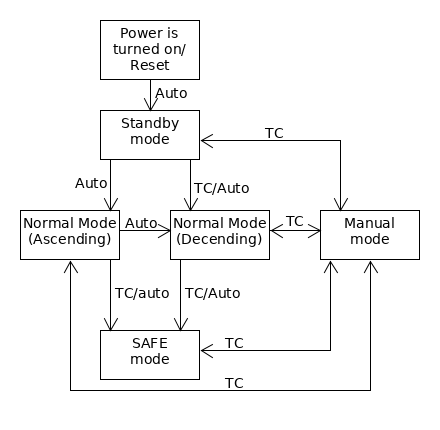
\includegraphics[scale=0.55]{4-experiment-design/img/state-diagram-V1-3.png}
    \end{align*}
    \caption{Process Diagram for the Modes.}\label{fig:modediag}
\end{figure}

In the sampling algorithm, it was necessary to keep track of the time because the bag could not be filled fully (it might burst). A simple library was used to keep track of the time from the start of the experiment.\par 

\item{Modularization and Pseudo Code}\\
\begin{figure}[H]
    \begin{align*}
        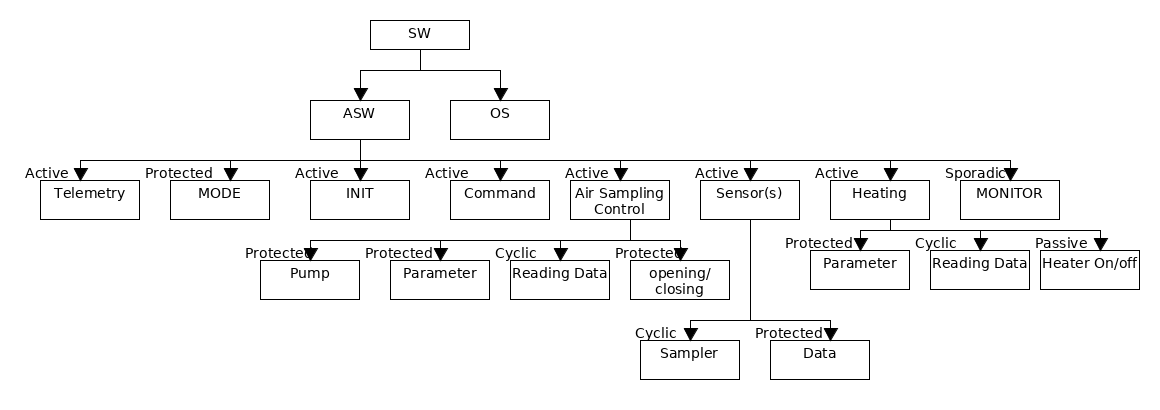
\includegraphics[width=1\linewidth]{4-experiment-design/img/sw_design_v1-8.png}
    \end{align*}
    \caption{Onboard Software Design Tree.}\label{fig:obtree}
\end{figure}

The software design was produced by using object oriented approach. The functionality of the experiment was divided into several objects and their children. The design tree is shown in Figure \ref{fig:obtree}.\\
\\
The Telemetry object was responsible to format the sensor/housekeeping data, and to transmit it. MODE was responsible for controlling the five modes of software. INIT initialized the necessary software. COMMANDS read the telecommands and executed their commands. The AIR SAMPLING CONTROL object had the four children objects. The first child was responsible for controlling the pump. The second child contained the parameters for the valves and pump. The third child read the data from the sensors, a fourth child was responsible for manipulating the valves.\\
\\
The SENSOR object had two children objects. One for sampling the sensors and another for recording and storing the housekeeping data. The HEATER object had three children objects. One for reading the temperature sensor data, another for deciding if the heaters should be turn on/off. And the third child for turning it on/off.\\ 
\\
The MONITOR object utilized a watchdog timer that caused an interrupt when it reaches 0. The watchdog did not get fed directly from by the end of the different tasks. Instead the tasks set a flag, if all the flags were set the watchdog got reset and the countdown started from the beginning. If the watchdog timed out before all the flags were set the monitor object reset the board.\\
\\
Each of the objects interacted with each others fulfilling mutually exclusive interaction. It meant that any shared variables could only be accessed by one object at time. This was important considering the program was fully automatic and to prevent unnecessary data lost. The objects interface diagrams and their sequence diagrams can be found in Appendix \ref{sec:appB} and \ref{sec:appC}.
\end{enumerate}
%\begin{figure}[H]
%    \centering
%    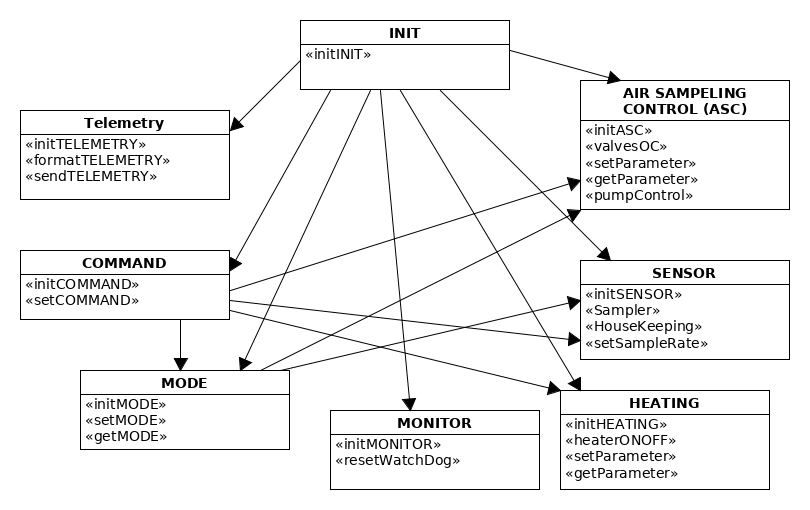
\includegraphics[width=1\textwidth]{4-experiment-design/img/hood-diagram-v1-0.png}
%    \caption{Hierarchic Object-Oriented Design of the software}
%    \label{fig:hood}
%\end{figure}
\subsubsection{Implementation}\label{sec:4.8.3}
The C/C++ programming language was used when programming the platform. Instead of Arduino IDE, PlatformIO IDE was used, other software was used if necessary. The software was functioning autonomously using a real-time operating system. FreeRTOS was chosen as the real-time operating system, which provided a feature to split functionality into several mutual exclusive tasks. These tasks were \begin{itemize}
    \item The Sampler task (periodic)
    \item The Reading task (periodic)
    \item heaterTask task (periodic)
    \item telecommand task (sporadic)
\end{itemize} 
Several libraries that were used:
\begin{itemize}
    \item FreeRTOS\_ARM.h (FreeRTOS specially port for ARM microprocessor like Due)
    \item ArduinoSTL.h (allows standard C++ functionality)
    \item RTCDue.h (keeps track of the time from the software start)
    \item Necessary Arduino libraries.
    \item DS1631.h (self made library)
    \item MS5607.h (self made library)
    \item Sensors libraries.
\end{itemize}


\raggedbottom